\documentclass[]{article}
\usepackage{graphicx}

%opening
\title{Annotated Bibliography}
\author{Kaushi Perera}

\begin{document}

\maketitle


\section{Ye, Z., Gwizdka, J., Lopes, C. T., \& Zhang, Y. (2017). Towards understanding consumers' quality evaluation of online health information: A case study. Proceedings of the Association for Information Science and Technology, 54(1), 838-839.}

In this case study the authors' intention has been to understand and investigate upon how consumers' evaluate quality of online health information. The approach of this study has been to use 'eye-tracking' and conducting 'retrospective interviews' in order to investigate different interface elements which are being used by consumers' to evaluate quality and also to investigate whether differences in individuals, such as eHealth literacy and personality have any influence on consumers' behaviour.     


\textbf{Method}

Twelve people have participated for this study. The study has been conducted in a lab with a personal computer and an ‘eye-tracking device’. The first task for the participants has been to fill questionnaires related to their demography, personality and e-health literacy questionnaires. Then all the participants have been given five predefined tasks related to health information search. For each of these predefined tasks, three preselected web pages have been provided. Then participants have been instructed to study each of these three web pages and to determine whether these web pages are recommendable to their family or friends. 

\textbf{Results}

The researchers have presented results for two out of twelve participants because it has been noticed that the ‘eye-movement patterns’ for these two participants have had a huge difference on one web page.

This particular web page has been related to the following scenario:

'Imagine that one of your friends is struggling with whether to have her teenage son receive an influenza vaccine. So you conducted an online search, these three web pages are among the pages that show up in the search results. After browsing each page, you will determine whether you want to share this page to your friend'

According to the resulted reported for these two participants it has been noted that their gaze plots (position, order and approximate time spent at fixating at locations) and their eye-movement patterns are almost exactly the opposite to each other. According to the gaze plot illustrations P1 has viewed the text-based web content as a F-shaped pattern. Also, it has been noticed that this participant’s fixations are mostly on the main text content with a reading focused on topical information. However, the other participant P2’s gaze plots are noticed to have an atypical pattern and this participant’s fixations have found to be scattered all over the web page, such as at the top, right side, bottom areas and a few in the main content area.    

The gaze plots for P1 and P2 are shown in Figure~\ref{fig1}

\begin{figure}[b!]
	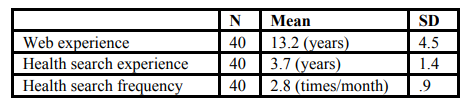
\includegraphics[width=0.8\textwidth]{Capture1.png}
	\caption{Gaze plots of P1(left) and P2(right). \label{fig1}}
\end{figure}      

The performance of this task for the two participants have been examined by considering information, such as the choice made on this page, time on task, time on page and count of links clicked on. The participants’ background information has also been examined, including their eHEALS and TIPI scores. Therefore, it has been identified that the first participant P1’s eHEALS score is considerably lower than P2 and also that P1 has spent a longer time on the task and on the web page itself when compared to P2.      

The two participants' task performance and background information are shown in Figure~\ref{fig2}

\begin{figure}[t!]
	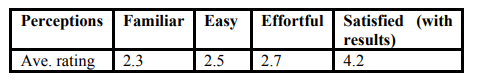
\includegraphics[width=0.8\textwidth]{Capture2.png}
	\caption{Task performance and background information. \label{fig2}}
\end{figure}  

The web elements which have been mentioned by these two participants as their preferences for evaluating the quality of the web page has also been noted during their RTA interviews.  

The preferred web page elements of the two participants are shown in Figure~\ref{fig3}

\begin{figure}[b!]
	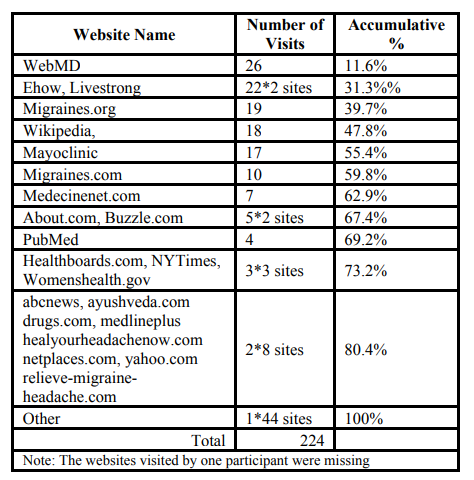
\includegraphics[width=0.8\textwidth]{Capture3.png}
	\caption{Preferred web page elements of each participant. \label{fig3}}
\end{figure} 

\textbf{Conclusion}

In conclusion it is said that different eye-movement patterns of consumers can be due to the several factors, such as demographic factors, familiarity with the health-related topic and health literacy. Finally, based on the observations of this study and collected data, the researchers have formulated a few hypotheses which are to be tested in future studies:

Consumers’ with comparably lower eHealth literacy are tend to:  

H1a. ‘spend more time on quality evaluation’
H1b: ‘rely more on relevance than on quality indicators’  

When considering health-related web page quality:

H2a: ‘Consumers with considerably lower eHealth literacy tend to rely more on the main content of a webpage than on quality indicators’
H2b: ‘Consumers with considerably higher eHealth literacy are able to take advantage of quality indicators’


\section{Lopes, C. T., \& Fernandes, T. A. (2016, September). Health Suggestions: A Chrome Extension to Help Laypersons Search for Health Information. In International Conference of the Cross-Language Evaluation Forum for European Languages (pp. 241-246). Springer, Cham.}

Even though consumers are tend to search health-related information via the Internet, lack of proper medical/scientific vocabulary and the use of languages with less information (Portuguese compared to English) have restricted users from accessing useful health information on the Web. Because the majority of the consumers are tended to use health-related web content and diagnosis information without properly assessing the quality or double checking the information with a medical professional, it is crucial to fill in the gaps for accessing health-related information.   

Although it is obvious that with more ‘medico-scientific’ terminology included in a query a consumer will be able to retrieve more detailed and scientific content, the utility of this information is highly dependent on the person’s domain knowledge. This is because more detailed and scientific information can be useful for a person with more expertise and a person with less domain knowledge will find this kind of information as not understandable. 
   
Therefore, it is important to consider both lay and medico-scientific terminology when assisting laypeople or consumers with health suggestions for their original queries. In this study the researchers have provided suggestions using two languages which are Portuguese and English depending on the language of the initial query. The health suggestions or assistance have been provided in search engines, covering three main search engines which are Google, Bing and Yahoo. The final aim of this study has been to present consumers with a mechanism which has the ability to assess them for finding higher-quality health-related contents that will also fit for consumers’ health expertise.      

\textbf{Health Suggestions}

The health suggestions have been implemented in Google Chrome as a ‘Google Chrome extension’. The reasons for choosing Google Chrome have been because the study is focused on extending browser’s functionality and then reaching the main three search engines, and also because Google Chrome is considered as the users’ preferred browser.   

The health suggestions have been presented to users as panel. The users have been allowed to perform actions, such as to ‘search for suggested queries; switch search engines; minimise/maximise the panel and close the panel’. Therefore, if a user clicks on a suggestion a new search has been performed or if a user clicks on a search engine’s icon, then the same search has performed in the relevant search engine. 

However, the panel has been only available when matches were identified between Health Suggestions and queries, in the data structures which have been used. This extension also has been facilitated with an options page. Users were able to navigate to the options page by clicking on an icon which was a ‘blue heart’ on the suggestions' panel. This options page has facilitated users to perform actions, such as ‘turning the extension on/off, (dis)allowing logging, opting for a local or remote database, specifying queries’ language or asking the extension to automatically detect it’.     

The Suggestions' panel and the Options page are shown in Figure~\ref{fig4} and Figure~\ref{fig5} respectively.

\begin{figure}[b!]
	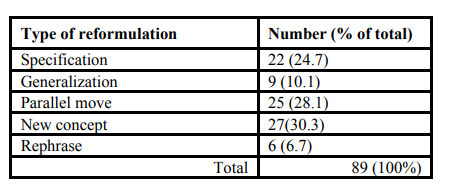
\includegraphics[width=0.8\textwidth]{Capture4.png}
	\caption{Suggestions' panel. \label{fig4}}
\end{figure}  


\begin{figure}[t!]
	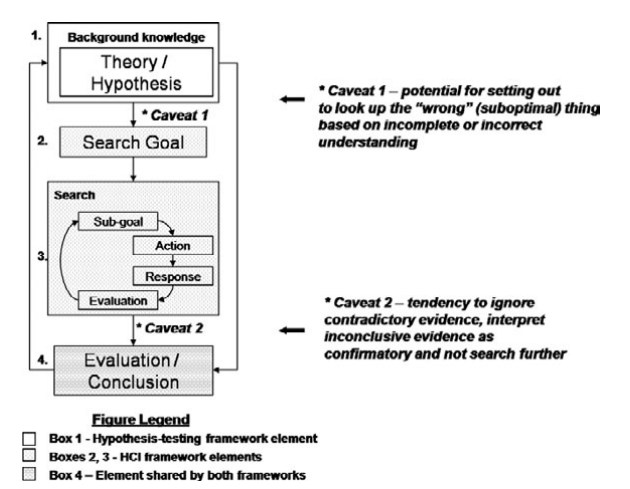
\includegraphics[width=0.8\textwidth]{Capture5.png}
	\caption{Options page. \label{fig5}}
\end{figure} 

This system has been consisted with two distinct modules, such as the suggestion engine and the login engine.
 
\textbf{Suggestion engine:} The responsibility of this engine has been to generate suggestions accordingly. As in this study suggestions are provided both in English and Portuguese, the researchers have used both English and Portuguese versions of the Consumer Health Vocabulary (CHV). In CHV everyday health-related terms are linked to technical terms which are used by health care professionals. Also, the extension is standalone because the users can use a local database except the remote database. 
      
The researchers have created two inverted indices for each language with the use of CHV. Each inverted index has been consisted with stemmed terms with their corresponding ‘inverse string frequencies (isf)’ and CHV string lists indicating where each stemmed term appears. As to determine the vocabulary of each term, CHV’s strings have been tokenized and the stop words have also been removed. In the rest of the terms letters have been reduced to lower case, the diacritics have been removed and those terms have also been stemmed.

According to the Suggestion engine architecture the first few steps are performed in the extension and the final few steps are able to be performed either in the extension or in the server. The majority of the steps of this process is performed in the extension to accomplish efficient response time. 

The suggestion engine architecture is shown in Figure~\ref{fig6}

\begin{figure}[b!]
	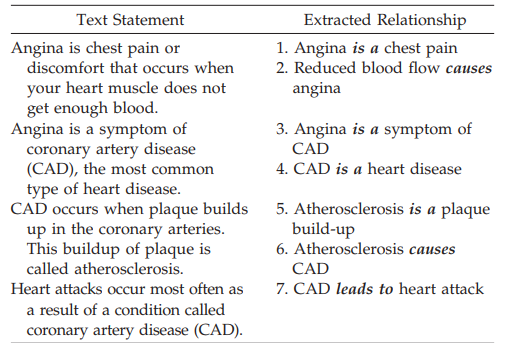
\includegraphics[width=0.8\textwidth]{Capture6.png}
	\caption{Suggestion engine architecture \label{fig6}}
\end{figure}   


\textbf{Login engine:} The responsibility of this engine has been to understand users’ search process by tracking different actions performed by users when searching for health-related information. The importance of doing this has been to further improve Health Suggestions provided to users. Therefore, this engine has focused on information, such as ‘query, search engine, search results, search engine’s related queries and the suggestions provided by the Health Suggestions; time spent on SERP and Health Suggestions’ panel; visited web pages: time on page and number of scroll events; clicks: on the extension’s panel, search results or any page hyperlink; copy/cut events; find events’. This logging engine has also consisted of two modules which are the extension and the server. However, this tracking of user actions is provided as an option where users are allowed to disable the tracking via the options page.     

\textbf{Experiment}

The Health Suggestions have been evaluated using four research questions:

(1) How are suggestions used? 
(2) Why are suggestions used?
(3) How do users assess the utility of the suggestions provided by the system? 
(4) Do the suggestions lead to a more successful search?

In order to determine the success of the search, the researchers have considered how many relevant documents have been saved by the users and users’ opinions about the success of the task. The researchers have recruited 36 students for their study. The percentage of the participants who have had a daily web searching frequency is identified as 19\% where the majority (81\%) of the participants’ have had search frequencies as more frequent than daily. 
   
If the participants’ satisfaction (how often they find what they are looking for) is scaled from 1 to 5:

4 participants (11\%): classification was 3
26 participants (72\%): classification was 4
6 participants (17\%): classification was 5

\textbf{Setup}

The participants have been divided in to two groups where one group has received assistance via Health Suggestions (assisted group) and the other group has not (unassisted group). However, it has been found that there has been no significant difference when considering the average search experience between the two groups despite the number of years searching the web or users’ self-assessment of success in web searching.
    
In order to determine the health topics, 20 people with no medical expertise, in a wide range of ages and education levels have been asked to state the health topic that they have most recently searched on the Web, and the health topics have been selected randomly using this information.

Each participant has been instructed to perform four tasks and they have been required to formulate 3 queries per task. Then the participants have been instructed to save the relevant documents from the top 10 results received for each query. At the end of each task, participants in the assisted group have been instructed to explain factors, such as how they used Health Suggestions (clicked on them, used terms from one of the suggestions, used terms from several suggestions), why the suggestions were considered useful and to assess the utility of the Health Suggestions.        

\textbf{Results}

How are suggestions used?
 
According to the user behaviour of the assisted group, it has been identified that in 27\% of the cases out of all the cases where suggestions have been provided for queries (71\%), the users have clicked on these suggestions. In 15\% of the cases users have used suggestions to extract terms and have included these terms in their next query. In 4\% of the cases users have extracted terms from several suggestions.
     
Why are suggestions used?

Five main reasons have been identified as the reasons for using suggestions. In 35\% of the cases, it is because they presented synonyms, in 37\% of the cases because they present alternatives in medico-scientific terminology, in 24\% of the cases because they suggest English terms and in 3\% of the cases because of the lay terminology. 

How do users assess the utility of the suggestions provided by the system? 

The utility has been scaled in a range of 1-3. Out of all the presented suggestions, 35\% have been considered useful, 33\% partially useful and the rest of 29\% as useless. 

Do the suggestions lead to a more successful search?

When considering the average number of documents which have been saved by users, it has been noted that the number has been significantly higher for the assisted group 16.3 when compared to the unassisted group 14.1. For the overall task success, a scale of 1-5 has been used and it has been noted that the assisted group has resulted in a lower median 4 when compared to the unassisted group 5 even though this is not considered as a significant difference.     

\textbf{Conclusion}

In conclusion, both lay terms and medico-scientific term suggestions in Health Suggestions are able assist laypeople in order to retrieve information which will also fit to their domain knowledge. Therefore, the utility of a multilingual and multi-terminology approach is important and useful in order to retrieve a huge number of relevant documents.   

\section{Silva, R., \& Lopes, C. (2016). The Effectiveness of Query Expansion when searching for Health related Content: InfoLab at CLEF eHealth 2016. In CLEF (Working Notes) (pp. 130-142).}

One of the biggest difficulties of consumers’ when searching for health-related information is the lack of knowledge in medical terminology. This problem directly influences when consumers/ users formulate queries and will also directly lead to the dissatisfaction of users (do not satisfy expectations of users’) regarding the retrieved information/ documents. Therefore, this study has focused on using query expansion as a technique to improve the initial queries issued by laypeople, so as to improve the overall retrieval performance. Query expansion is known as the process of ‘supplementing the original query with additional terms’.    

\textbf{Method}

\textbf{Task Description:} The aim of the overall task has been to evaluate systems which support people (specially patients) to understand and search for health-related information. This has been done by evaluating a ranked list of documents which have been retrieved by issuing patients’. A TREC-style evaluation process has been conducted in this study by using the provided test collection. This task has been split into three sub tasks and in this study the ad-hoc search and the query variation are considered.  
    
\textbf{Document Collection:} The document collection for these tasks has been the ClueWeb12 B13 Dataset. This collection of documents has excluded documents which was not in the top 90\% of pages least likely to be spam and any documents which have appeared in the blacklist provided by a URL blacklist service. 

\textbf{Queries:} The query generators have been presented with health consumer posts which are from health web forums. Then the query generators have created query based on these initial user posts and by making several variations to the same condition.  
 
\textbf{System Description:} For this study ‘Terrier’ has been used because it has the ability to implement indexing and retrieval functionalities. Also, it facilitates for rapid development and evaluation of retrieval applications. In this study the Terrier index has been provided to all the participants in order to make sure that all the participants have access to the same index. This has made it easier to compare the final results of the participants. 

\textbf{Retrieval Approaches}

Query expansion has been the main approach used in this study. Different sources and methodologies have been used to determine which terms to be added while performing the query expansion.   

The summary of Query expansion approaches used in this study are shown in Figure~\ref{fig7}

\begin{figure}[b!]
	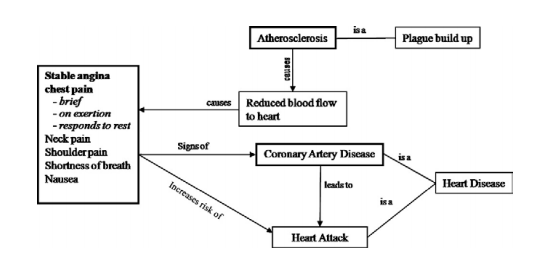
\includegraphics[width=0.8\textwidth]{Capture7.png}
	\caption{Query expansion approaches \label{fig7}}
\end{figure}   

\textbf{Baseline}

The BM25 term weighting model has been used in this study for scoring and ranking medical documents. This Okapi BM25 is a ranking function which is used by search engines to rank matching documents by considering their relevance to an issued search query.      

The equation to calculate a document's relevance score based on the BM25 term weighting model is shown in Figure~\ref{fig8}

Q: a query 
D: a document
TF: the number of a given term qi in the document D
|D|: the size of the document in words 
avgdl: the average size of a document
k1 and b: Free parameters. Usually are chosen in the absence of an advanced optimization as,

k1 ∈ [1.2; 2.0] b = 0.75

\begin{figure}[t!]
	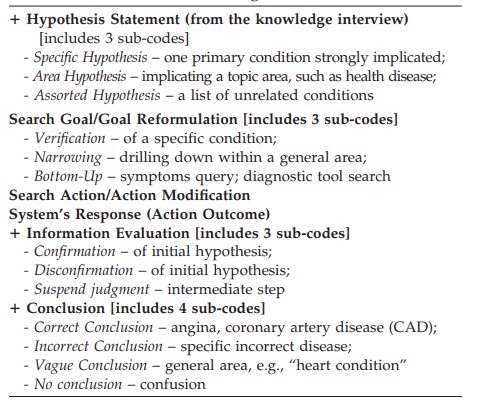
\includegraphics[width=0.8\textwidth]{Capture8.png}
	\caption{Relevance score of a document \label{fig8}}
\end{figure} 

\textbf{Pseudo Relevance feedback}

Pseudo Relevance Feedback is one of the methods which is used for query expansion. The top documents retrieved by the baseline have been used to modify queries. The modification is done by reweighting the existing query terms in order to determine which useful terms to be added and which useless terms to be deleted from the query. Then the modified query will be issued with the intention of retrieving relevant more documents than the original query.
 
Terrier facilitates for two different models in order to apply the pseudo relevance feedback method: the Bose-Einstein and the Kullback-Leibler Divergence. The BoseEinstein model calculates the weight of terms as shown in Figure~\ref{fig9}

\begin{figure}[b!]
	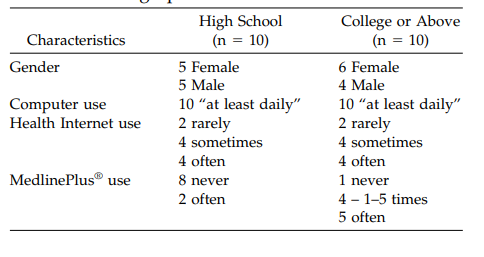
\includegraphics[width=0.8\textwidth]{Capture9.png}
	\caption{The BoseEinstein model \label{fig9}}
\end{figure} 

tfx : the frequency of the query term t in the top-ranked documents
tfc: the frequency of term t in the collection
N: is the number of documents in the collection

The Kullback-Liebler Divergence: This approach computes the divergence between the 'probability distribution of terms in the whole collection' and the 'top ranked documents which have been obtained using the original query'. Therefore, the most likely terms which can be used for expanding the query are the terms which have a higher probability in the top ranked set and a lower probability in the whole collection. 

The Kullback-Leibler Divergence formular is shown in Figure~\ref{fig10}

t: term
Pr(t): the probability of t estimated from the top retrieved documents relative to a query (R)
Pc(t): the probability of t estimated using the whole collection
 
For the approach of pseudo relevance feedback, two runs have been performed to identify which one of this models
is able to provide better results.   

\begin{figure}[t!]
	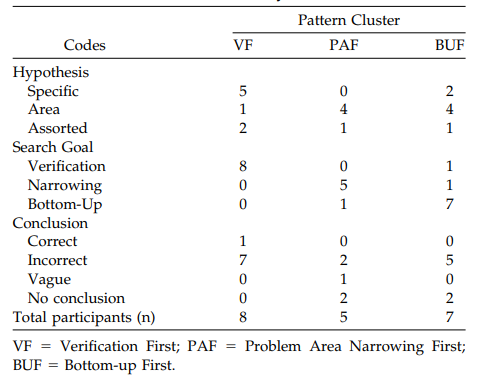
\includegraphics[width=0.8\textwidth]{Capture10.png}
	\caption{The Kullback-Leibler Divergence model \label{fig10}}
\end{figure}

\textbf{Query expansion using the Medical Text Indexer}

The task of the NLM Medical Text Indexer (MTI) is to combine human NLM Index Section expertise with Natural Language Processing technology. This facilitates for curating the biomedical literature in a more efficient and consistent manner. The MTI also provides indexing recommendations based upon the Medical Subject Headings (MeSH) vocabulary since 2002.    

When the queries are processed by MTI, it will link the query text to the MeSH vocabulary which will provide additional related concepts. These concepts are highly likely to be important for the retrieval process. However, because MTI results are machine generated, there is possibility for generating irrelevant concepts.  
  
In this study all the concepts which were identified and suggested by the MTI have been appended to the original query.  

\textbf{Query expansion using Wikipedia} 

Because people are tend to improve Wikipedia by making changes by themselves, it is likely that it contains medical terms in lay language. Therefore, Wikipedia is considered as a prominent source of online health information. In this study, two methods have been used to obtain terms for query expansion while using Wikipedia as the base. The first method has been used to extract 'the most frequent terms' from Wikipedia articles. The second method has considered the Wikipedia as a directed graph and has used it to determine similar articles in order to extract terms from the titles of these articles.        

\textbf{1. Term frequency} 
 
The MediaWiki action API has been used to search for articles which have best matches to the concepts obtained via the MTI. Out of these Wikipedia pages, some pages may not be relevant to health, therefore all the pages which does not contain an infobox (contains information about the category of the page) has been removed. An example of an infobox is shown in Figure~\ref{fig11}. In this approach the 5, 10 and 15 most frequent terms for each article has been chosen. Other than that the researchers have also considered 'all articles found with the MTI concepts' and 'only the articles considered health-related'.   

\begin{figure}[t!]
	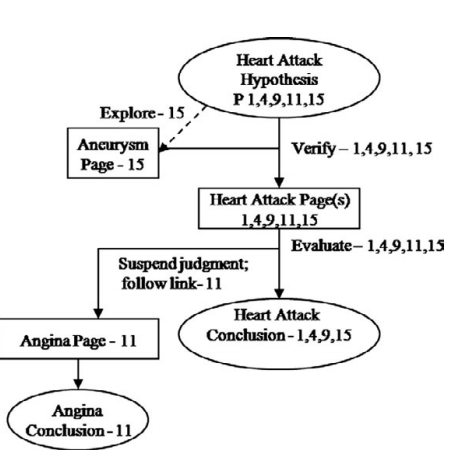
\includegraphics[width=0.8\textwidth]{Capture11.png}
	\caption{Wikipedia Asthma Infobox \label{fig11}}
\end{figure} 

\textbf{2. Link analysis}

As mentioned above when considering one Wikipedia article, it can refer to other Wikipedia articles via hyperlinks. When consider hyperlinks which are targeted at other Wikipedia articles, these Wikipedia articles can be represented as a direct graph of articles. For each article there can be a set of incoming and outgoing links.   

When using Wikipedia direct graph for retrieving articles for the expansion process, this may retrieve a huge number of irrelevant articles. As a solution to this the 'Jaccard similarity coefficient' has been used to measure the similarity between sample sets. Jaccard similarity coefficient is calculated by dividing the 'size of the intersection' by the 'size of the union' of the sample sets.       

I: Incoming links 
O: Outgoing links

The Jaccard similarity coefficient equation is shown in Figure~\ref{fig12}

\begin{figure}[t!]
	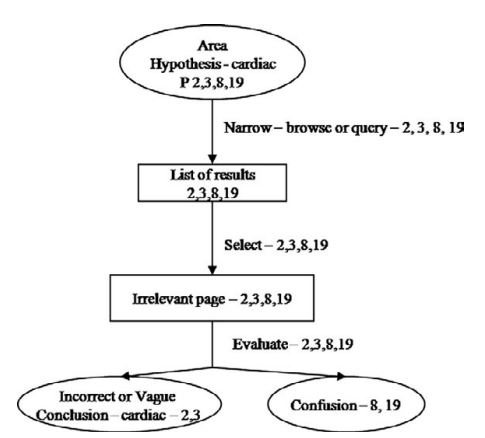
\includegraphics[width=0.8\textwidth]{Capture12.png}
	\caption{The Jaccard similarity coefficient \label{fig12}}
\end{figure} 

Therefore, all the titles of the articles which have had a Jaccard similarity coefficient greater than 0.25, 0.50 and 0.75, have been added to the original query. In addition, 'all articles found with the MTI concepts' and 'only the articles considered health-related' have also been considered in this approach.   

\textbf{Query expansion using MedlinePlus} 

As the world’s largest medical library, MedlinePlus consists of information regarding diseases, conditions, and wellness issues which are in lay language. The information from the infoboxes have been used to access corresponding MedlinePlus pages. Because MedlinePlus pages consist of several sections, for this study the sections, such as the Causes, Symptoms, Treatment, Possible Complications and Alternative Names sections have been taken into account for the query expansion process. The top 5, 10 and 15 most frequent terms have been obtained from each of these relevant sections. Almost all of the term which have been included in the Alternative Names section have been used.    

\textbf{Query expansion using the ICD-10}

ICD-10 is a medical classification list provided by the World Health Organization (WHO). This consists of codes for diseases, signs and symptoms, abnormal findings, complaints, social circumstances, and external causes of injury or diseases. In this approach also the information from the infoboxes have been used to access corresponding information from the ICD-10 pages. ICD-10 pages also contain information about diseases or symptoms related to the initial search concept. Therefore, the terms in this related information have also been used for the query expansion process. The top 5, 10 and 15 most frequent terms has been chosen from the ICD-10 pages to be appended with the original query.        

\textbf{Query expansion using Latent Dirichlet Allocation over Wikipedia}

The main purpose of using this Latent Dirichlet Allocation has been to extract or generate different latent topics which are being represented by text. Therefore, each word on the text is tend to peak towards or represent one of the possible topics. The texts considered here are the Wikipedia articles representing different MTI concepts.  

An example of LDA applied to a text is shown in Figure~\ref{fig13}. In this example it has generated four topics for the text and have separated words which represent each topic. 

\begin{figure}[t!]
	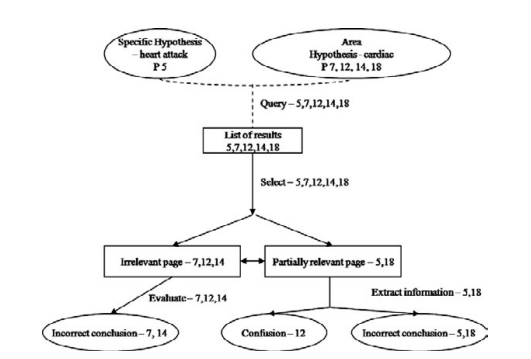
\includegraphics[width=0.8\textwidth]{Capture13.png}
	\caption{An LDA example which generates four topics \label{fig13}}
\end{figure}

In this study different combinations of number of topics and number of words, such as a combination of 3 topics with 1, 5 and 10 words, and 1, 5 and 10 topics with 5 words have been tested 
 
\textbf{Query expansion using Unified Medical Language System} 

The Unified Medical Language System (UMLS) contains approximately 900,000 biomedical concepts in it. In order to be used in the expansion process, terms have been extracted from the UMLS definitions which are related to the MTI concepts. For this study researchers have chosen the top 5, 10 and 15 most frequent terms from the UMLS definitions in order to be appended to the original query.   

\textbf{Readability}

Readability measures the ‘difficulty of understanding a passage of text’. For this study three readability metrices have been used which are SMOG, FOG and Flesch-Kinciad. These metrices represent the ‘educational grade level’ which is needed to understand a document.   

\textbf{The SMOG readability measure} is calculated for a document with 30 sentences. In a case where the document is longer than 30 sentences, the first 10 sentences, the middle 10 sentences, and the last 10 sentences will be used for the calculation. In a case where the document is shorter than 30 sentences certain rules and conversion tables will be used to perform the calculation.  

The SMOG readability measure formula is shown in Figure~\ref{fig14} 

\begin{figure}[b!]
	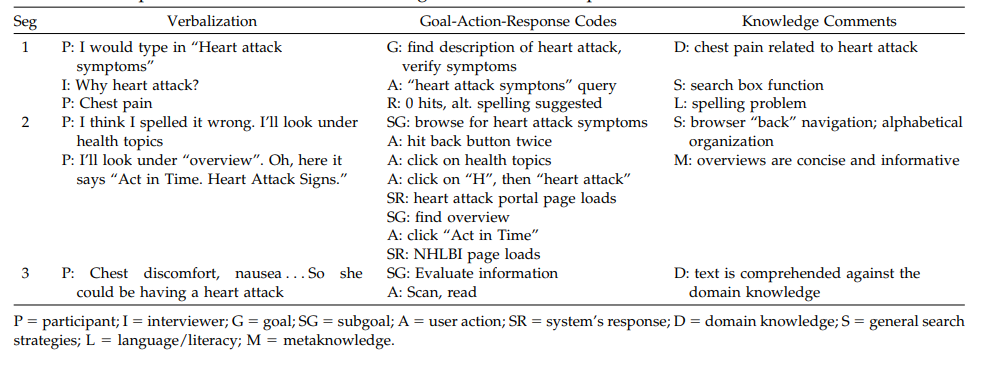
\includegraphics[width=0.8\textwidth]{Capture14.png}
	\caption{The SMOG readability measure formula \label{fig14}}
\end{figure}

The FOG Index readability formula which is known as suitable for secondary and older primary age groups considers the Average Sentence Length (ASL) which is the values obtained by dividing the number of words from the number of sentences and the Percentage of Hard Words (PHW) which is obtained by selecting the words of three or more syllables.    

The FOG Index readability formula is shown in Figure~\ref{fig15}

\begin{figure}[t!]
	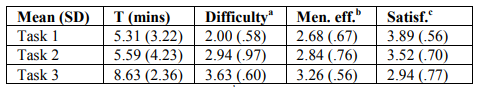
\includegraphics[width=0.8\textwidth]{Capture15.png}
	\caption{The FOG Index readability formula \label{fig15}}
\end{figure}

The Flesch-Kincaid formula takes into account the Average Sentence Length (AST) which is the number of words divided by the number of sentences and the Average number of Syllable per Word (ASW) which is the number of syllables divided by the number of words. 
    
The Flesch-Kincaid formula is shown in Figure~\ref{fig16}

\begin{figure}[b!]
	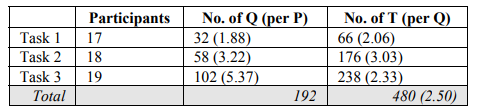
\includegraphics[width=0.8\textwidth]{Capture16.png}
	\caption{The Flesch-Kincaid formula \label{fig16}}
\end{figure}

For this study, a re-rank method has been used to combine readability metrics and the relevance  scores obtained from the Terrier. Three formulas have been used to combine these values.
 
The three formulas used for combing values are shown in Figure~\ref{fig17}

\begin{figure}[t!]
	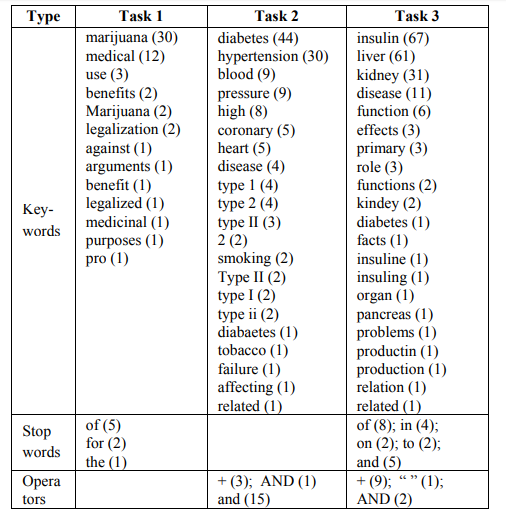
\includegraphics[width=0.8\textwidth]{Capture17.png}
	\caption{The three formulas used for combing values \label{fig17}}
\end{figure}

For the third formula ‘th’ is defined as a readability threshold where documents that have a readability score below th are considered as readable and documents that have a readability score above th are considered as unreadable.

In this study each run has been re-ranked using one of the readability metrics and one of the combination formulas. This has generated a total of 9 different variants for each of the runs.

\textbf{Results}

For the ad-hoc search sub task each query has been treated individually by ignoring all the other query variations. For the query variation sub task each group of query variations have been treated as one query. The results have been compared with the baseline for each sub task. The results have also been evaluated for the submitted runs.  

\textbf{Submitted Runs}

Three runs have been submitted in this study, including the baseline, ‘Wikipedia Link Analysis with a Jaccard similarity coefficient above 0.50 by using health-related Wikipedia articles’ and the ‘Latent Dirichlet Allocation with 3 topics and 5 words’. For the re-ranking of these runs the SMOG readability metric and the second combination formula have been used. 

\textbf{Conclusion}

However, because the relevance and readability assessments for the test collection have not been available the authors have not been able to make conclusions regarding the results which have been obtained by following different approaches.   

\section{Graham, L., Tse, T., \& Keselman, A. (2006). Exploring user navigation during online health information seeking. In AMIA Annual Symposium Proceedings (Vol. 2006, p. 299). American Medical Informatics Association.}

This study has been focused on investigating user navigation behaviour patterns while seeking for online health-related information. The navigation behaviour patterns have been investigates at the National Library of Medicine (NLM) consumer health Web site, ClinicalTrials.gov. Transaction log analysis (TLA) is the method which has been used in this study to extract data from log files in order to investigate online user navigation behaviour. Therefore, this investigation has focused on online search behaviour, query failures, navigation, and browsing strategies. The other user actions, such as clicking on links, initiating queries, and other task-oriented actions (logging into a system) have also been taken into account for this research.     

\textbf{Methodology}

ClinicalTrials.gov log data has been used for this study. 

\textbf{Parsing:} Log data has been parsed and converted into data structures which have been written using XML. These data structures have included:

\textbf{Client:} A unique IP address which is associated with one or more session

\textbf{Session:} A set of sequential actions performed during an information seeking task

\textbf{Request:} Represents a user action and its corresponding Web server response 

\textbf{Preprocessing:} A Java program has been to correct erroneous session data, filter out Web crawlers and to insert the rest of the log data into a MySQL database. Temporary cookies have been used to estimate session boundaries in the client’s web browser. The session which are 10 minutes apart have been conflated into one session and any single session which has requests 30 minutes or greater apart have been split into two sessions. The sessions which have not included referring page or browser type information have also been filtered.           

Analysis: High-level Web usage statistics, such as page reviews and referral frequencies have been assessed in this study. In addition, page transitions and navigation path frequencies have also been assessed in this study. The data analysis has been performed by aggregating Web pages into functional categories.  

The functional categories of Web pages are shown in Figure~\ref{fig18}

\begin{figure}[t!]
	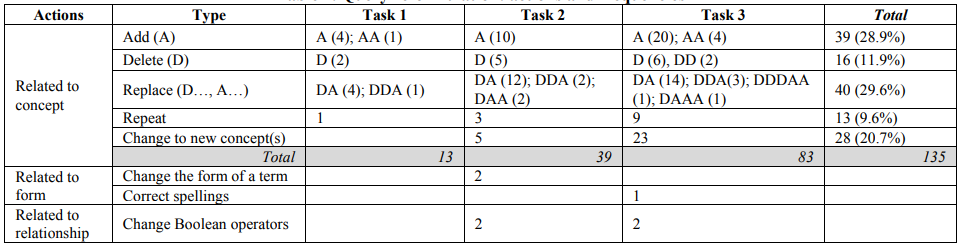
\includegraphics[width=0.8\textwidth]{Capture18.png}
	\caption{Categories for page-based analyses \label{fig18}}
\end{figure}

The frequency of users moving from one page to another within sessions has been computed and a single-transitions table has been built using this information. 
 
Algorithms have been used to determine navigation paths. These paths have been “condensed” by folding ‘multiple consecutive page occurrences’. Folding has been done as ‘page-plus-fold marker’. For instance, ‘View Results → View Study → View Study folded into View Results → View Study(N)’. Then the folded paths have been clustered and have been analysed manually.  
  
\textbf{Pilot User study}

Two hypothetical scenarios which are ‘sleep apnea’ and ‘Parkinson’s disease’ have been used to investigate consumers’ search behaviour for clinical trials. Participants were supposed to search for information for either one of the scenarios assigned to them. They have been allowed to search any online resource as their choice or thinking aloud. TechSmith’s Morae™ has been used to capture user-computer interactions and verbal responses. It is considered as the session is ended when participants decide that relevant information had been found or they need to determine that relevant information did not exist online. Researchers have analysed click stream data, participant comments, usage statistics, and navigation data.

After parsing and preprocessing the log data, the remaining log data, including 1.4 million sessions―5.5 million requests for 675,000 unique clients have been analysed. It has been found that ‘View Study pages’ which contained trial summaries are the most frequently requested and have been the most common entry and exit points to ClinicalTrials.gov. 

ClinicalTrials.gov usage statistics are shown in Figure~\ref{fig19}

\begin{figure}[t!]
	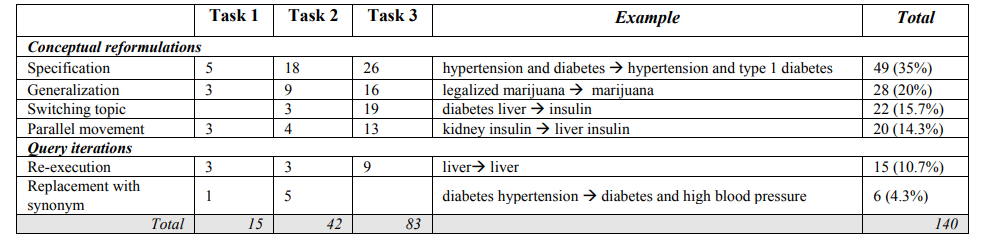
\includegraphics[width=0.8\textwidth]{Capture19.png}
	\caption{ClinicalTrials.gov usage statistics \label{fig19}}
\end{figure}

External Web sites, such as search engines and government sites have been the initiation point for 69\% out of all the sessions. The top five referring Web sites which represents 66\% of all referrals are shown in Figure~\ref{fig20}

\begin{figure}[t!]
	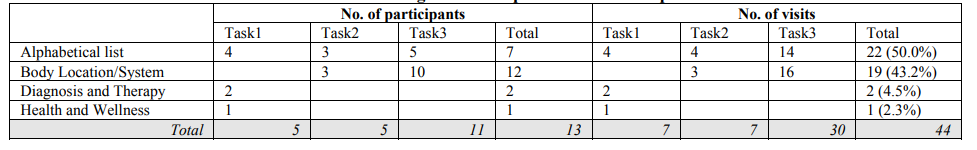
\includegraphics[width=0.8\textwidth]{Capture20.png}
	\caption{Top ClinicalTrials.gov referrers \label{fig20}}
\end{figure}

It has been found that there are three pages which serve as Web site entry and exit points. These pages are View Study, View Results and Opening Screen (homepage). Also, it has been found that there are three most frequent moves between pages which are ‘users viewing two studies in a row, viewing a study and exiting, and clicking on a specific study in the results list’. According to this investigation the users have shown a behaviour where they have only moved between a limited set of pages.
      
By analysing the 100 most frequent user paths researchers have been able to identify 8 common user navigation patterns. These patterns also reveal that users were generally tend to access ClinicalTrials.gov directly via ‘View Study’ pages. 
    
The path patterns are shown in Figure~\ref{fig21}

\begin{figure}[b!]
	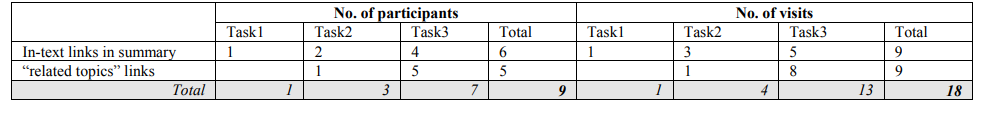
\includegraphics[width=0.8\textwidth]{Capture21.png}
	\caption{ User path pattern frequencies \label{fig21}}
\end{figure}

\textbf{Pilot User Study}

According to the results obtained from 7 lay consumers, 5 out of 7 consumers have viewed at least one page at ClinicalTrials.gov during their session.  

The navigation results for five participants are shown in Figure~\ref{fig22}

\begin{figure}[t!]
	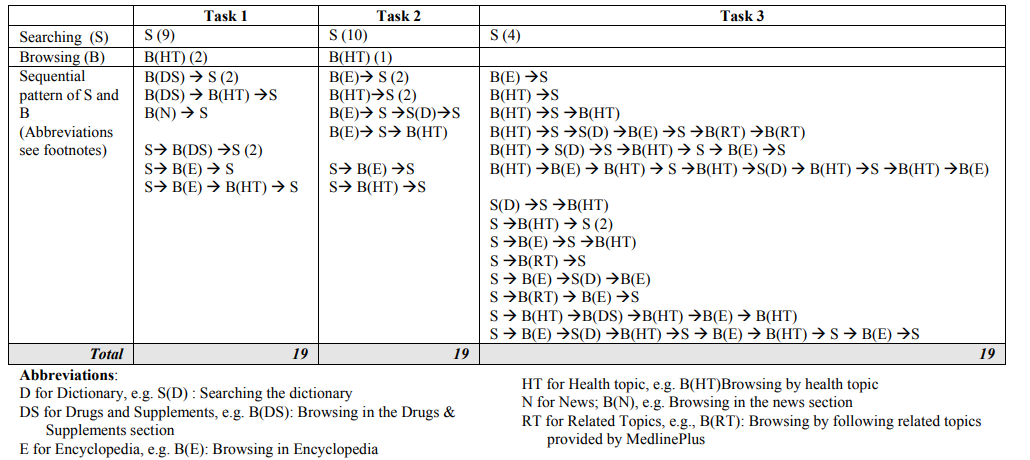
\includegraphics[width=0.8\textwidth]{Capture22.png}
	\caption{Overview of navigation actions at ClinicalTrials.gov by participant (n=5)  \label{fig22}}
\end{figure}

Out of the five participants who used ClinicalTrials.gov it has found that two of them have referred directly from search engines, another two from MedlinePlus and one from a non-profit health Web site. It has been also noted that participants most frequently entered and exited at the View Results in contrast to the TLA data where View Study page has been found as the main entry/exit point. 
  
The participants have judged the relevance of the Web sites by name recognition, “dot-gov” domains and keywords.   

Overall all participants have been satisfied with what they have found, therefore, have felt that they have found relevant and useful information.  
 
When the Web sire entry and exit points have been compared between the pilot user study and the log data, they both have shown similar structure of entry and exit points. As for the log data, the pilot user study also has shown that most moves have been occurred within the pages which are Opening screen, view results and view study. It has also been revealed that external Web sites, such as search engines direct users to results pages and individual studies. 

\textbf{Discussion}

According to the TLA log data a few user online navigation activities at ClinicalTrials.gov have been identified:

View Study (40\%) has been identified as the most frequently viewed page, followed by the View Results page (25%)
Users enter the site at a study level (39\%) which is more often than the homepage (24\%)
A majority of users (69\%) have been referred via external Web sites, including Google (41\%), other NIHsponsored sites (18\%), and other search engines (7\%)

The most common user session has been identified as viewing one or more View Study pages (40\%), followed by viewing a View Results page and clicking on a study (View Study) or simply viewing a results list/ View results page (9\% each)

In contrast to the initial expectations of the Web designers, it has been found that, majority of the users do not enter from the home page even though there are detailed menu options provided on the homepage, are tend to directly use the search and browse features provided by the site and are tend to spend time exploring the site and refining search queries for their information needs. 

It has been noticed that there is an increasing use of search engines, such as Google and therefore, the most ‘relevant’ pages indexed by search engines are tend to be exposed the most and also own the most direct visits. When considering the ClinicalTrials.gov, the most frequently visited pages are the View Study pages and View Results pages.  

It is noted that users do not use other available site features, such as ‘Search within results’ and ‘Resources’. This maybe because of the reason that users are not aware of the highly relevant information that might be accessible at the site.

Because most users do not enter a site via its Home Page, links to background information and other search features should be placed on lower-level pages which are been directly accessed by the users. This has the ability to increase the chance of users reaching related information. Also, the availability of visible local maps have the ability to retain users on the Web site.  

\textbf{Pilot User Study:}

It has been found that when the search query contained general terms users are tend to navigate to View Results page and when the search query contained specific terms or were complex queries, then the users are tended to navigate to View Study pages.      

\textbf{Conclusion}

According to the investigation which has been performed to understand user navigation on a consumer health Web site, ClinicalTrials.gov using the TLA log data, it has been found that the majority of users are tend to refer to low-level pages (View Study) from external Web sites, such as search engines. 

\section{Thenmozhi, D., Mirunalini, P., \& Aravindan, C. (2016). Decision Tree Approach for Consumer Health Information Search. In FIRE (Working Notes) (pp. 221-225).}

CHIS@FIRE2016 is a shared Task on Consumer Health Information Search (CHIS) which is collocated with the Forum for Information Retrieval Evaluation (FIRE). This CHIS track is consisted with two main tasks and this study is focused on the first task which is given a Consumer Health Information Search query and document associated with this query, determine whether the sentences included in this document are relevant to the CHIS query or not. The sentences are considered as relevant if they are useful and able to provide the answer to the query.  Therefore, in brief this study’s focus has been to categorize health care information retrieved from a query into two categories, such as relevant and irrelevant, using a machine learning approach.     

\textbf{Methodology}

A supervised approach has been used in this study. A few steps have been followed to create a decision tree.

1.	Preprocessing the given text
2.	Feature selection or extracting features for training data
3.	Use the selected features of training data to build a model using a classifier 
4.	Predict the class label for the instance either as “relevant” or “irrelevant” using the decision tree model

\textbf{Preprocessing:} By removing punctuations (‘, -) and by replacing apostrophes (n’t). Then the terms have also been annotated with parts of speech, such as noun, verb and adjective. Noun information and adjectives have been used to extract features.  

For instance, in the sentence ‘Skin cancer is more common in people with light coloured skin who have spent a lot of time in the sunlight’ nouns such as skin, cancer, sunlight and adjectives, such as light coloured has been considered similarly important. Therefore, all the nouns and adjectives have been chosen as features from the training data. In order to prepare the final feature set all the duplications from the extracted terms have been removed. 
    
Machine learning approach has been consisted of two variations which are:

1.	Approach without feature selection
2.	Approach using χ 2 feature selection

\textbf{Approach without feature selection:} The linguistic features have been used without explicit feature selection. The model has been built using the training data. Researchers have used a decision tree based classifier known as J48 to build this model. This classifier has used an algorithm called C4.5 to represent classification rules. Then the features vector of training data has been used to extract features from the test data with unknown labels. Then the built model has been used to predict labels for the test data instances.

\textbf{Approach using χ 2 Feature Selection:} Since all the features extracted from the training data may not be important for the classification, in this approach a chi-square value has been computed for selecting  important features from the linguistic features. The average or maximum χ 2 statistic value has been used to select the features which have strong dependency on the categories. Therefore, for each feature the occurrence or non-occurrence of each feature in relevant and irrelevant instances have been determined. 

Feature-Category Contingency Table for a feature shown in Figure~\ref{fig23}

O(fi, C): denotes the number of instances that contain the feature fi belong to category C
O(fi, ¬C): denotes the number of instances that contain the feature fi and are in not in category C 
O(¬fi, C): denotes the number of instances that does not contain the feature fi but belong to category C
O(¬fi, ¬C): denotes the number of instances that neither contain the feature fi nor belong to category C

\begin{figure}[b!]
	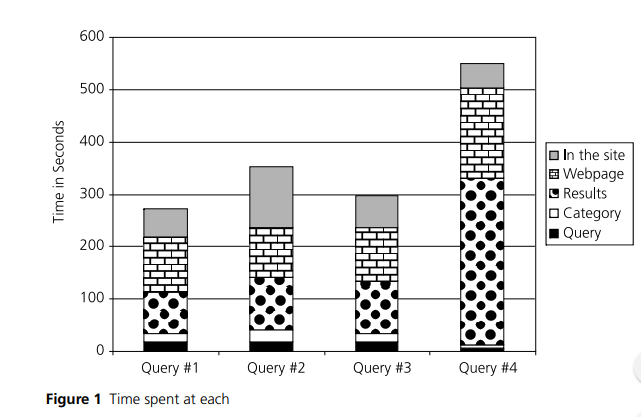
\includegraphics[width=0.8\textwidth]{Capture23.png}
	\caption{Feature-Category Contingency Table \label{fig23}}
\end{figure}   

The expected frequency for each feature has also been calculated with the use of observed frequency. The equation to calculate the expected frequency is shown in Figure~\ref{fig24}

i: represents whether the feature fi is present or not
j: represents whether the instance belongs to C or not
n: the total number of instances

\begin{figure}[t!]
	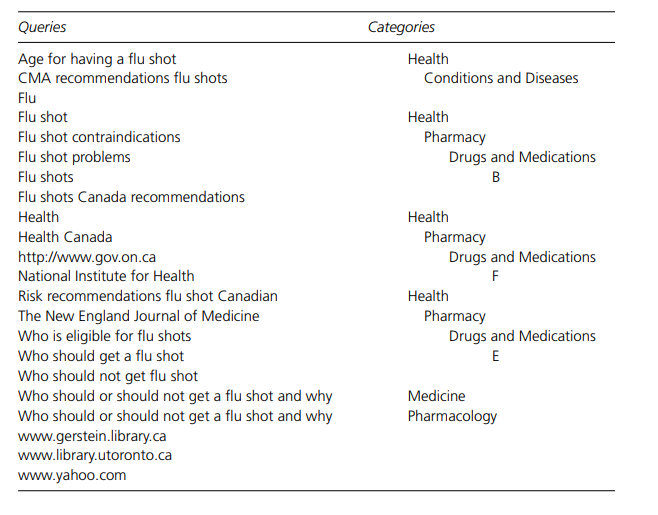
\includegraphics[width=0.8\textwidth]{Capture24.png}
	\caption{Expected frequency equation \label{fig24}}
\end{figure}   

Then expected frequencies which are E(fi, C), E(fi, ¬C), E(¬fi, C) and E(¬fi, ¬C) have also been calculated using the expected frequency equation.

Then χ 2 statistical value has been calculated for each feature to compare and determine whether each feature has a dependency on the categories.  

The equation for calculating χ 2 statistical value is shown in Figure~\ref{fig25}

\begin{figure}[b!]
	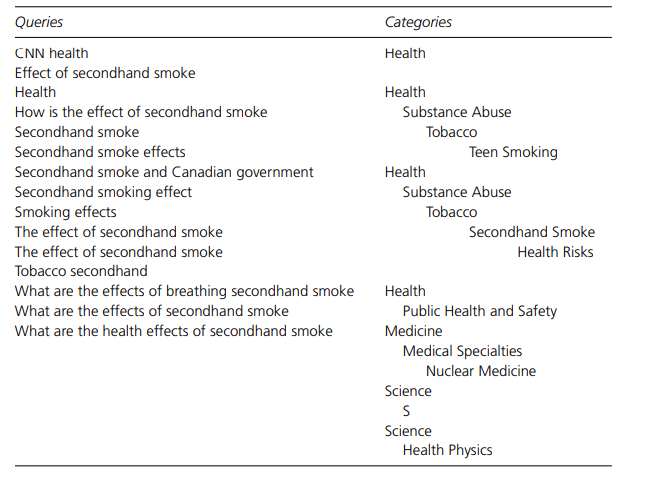
\includegraphics[width=0.8\textwidth]{Capture25.png}
	\caption{χ2 statistical value equation \label{fig25}}
\end{figure} 

Therefore, features whose χ 2 stat value is greater than χ 2 crit(α=0.05,df=1) : 3.841, has been considered as significant features and have been used to build the model. 

\textbf{Implementation}

The data set which has been used for the implementation has consisted of five queries and training and test data  for each query. 

This information is shown in Figure~\ref{fig26}

\begin{figure}[t!]
	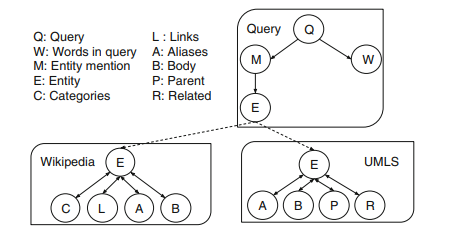
\includegraphics[width=0.8\textwidth]{Capture26.png}
	\caption{Data Set for CHIS task \label{fig26}}
\end{figure} 

\textbf{Approach without Feature Selection}

All the given sentences have been annotated using a technique called Stanford POS tagger. 

For instance, for the sentence ‘Skin cancer is more common in people with light coloured skin who have spent a lot of time in the sunlight’, skin, cancer, common, people, light, time, sunlight have been extracted as features. The features have also been lemmatized to bring the features to their root form.

The number features extracted for each query are shown in Figure~\ref{fig27} 

\begin{figure}[b!]
	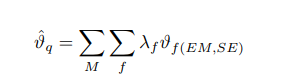
\includegraphics[width=0.8\textwidth]{Capture27.png}
	\caption{Data Set for CHIS task \label{fig27}}
\end{figure} 

\textbf{Approach using χ 2 Feature Selection}

The number of features selected for each of the queries using this statistical method are also shown in Figure~\ref{fig27} 

The size of the decision trees in terms of number of nodes are shown in Figure~\ref{fig28} 

\begin{figure}[t!]
	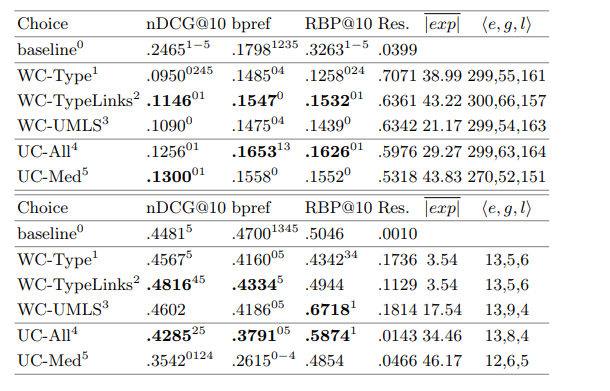
\includegraphics[width=0.8\textwidth]{Capture28.png}
	\caption{Size of the Tree\label{fig28}}
\end{figure} 

It has been noticed that the number of nodes for the χ 2 feature selection tree is considerably lower than the number of nodes for the tree without feature selection. By applying a k-Fold paired t-test it has shown that the reduction in size of the tree for χ 2 feature selection is statistically significant. 

\textbf{Results}

The 10-fold cross validation has been performed on training data for both methodologies to identify the cross-validation accuracies for each query. 

The cross-validation accuracies for each method are shown in Figure~\ref{fig29} 

\begin{figure}[b!]
	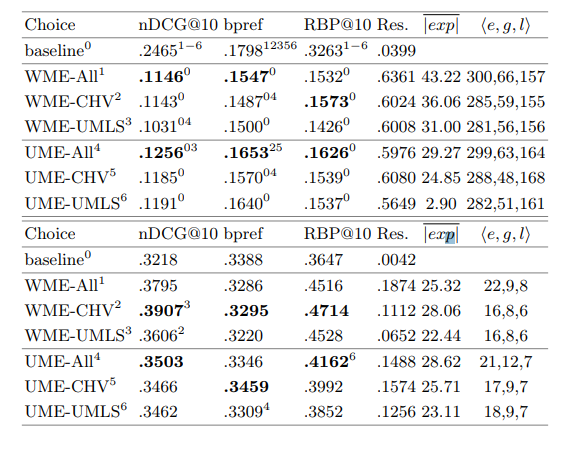
\includegraphics[width=0.8\textwidth]{Capture29.png}
	\caption{Size of the Tree\label{fig29}}
\end{figure} 

When the evaluation of test data is compared between the two methods, it has been noticed that χ2 feature selection method has had a 2.23\% higher accuracy when compared to the method without feature selection. 

Test data accuracy for the queries are shown in Figure~\ref{fig30}

\begin{figure}[t!]
	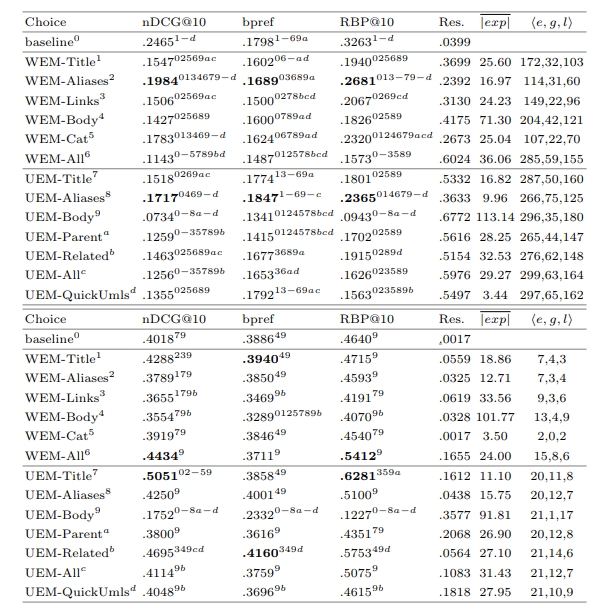
\includegraphics[width=0.8\textwidth]{Capture30.png}
	\caption{Size of the Tree\label{fig30}}
\end{figure}   

By using a k-Fold paired t-test it has been shown that improvement in performance for the χ2 feature selection method is statistically significant. By using a Mcnemar test across all data sets the researchers have confirmed that feature selection approach has the ability to significantly reduce the size of the model without compromising the performance.

\textbf{Conclusion}

Since this approach specially the one with χ2 feature selection has shown positive results in categorising health related documents as relevant and irrelevant, this technique can be used for filtering irrelevant health related documents prior viewing results to consumers which will help consumers to retrieve more relevant health related documents according to their issued query.  



\end{document}